\subsection{Probing for the Great Firewall}
Before probing for the GC, I first verified that I was able to reproduce the results of Marczak et al.~\cite{Marczak2015} with respect to the GFW.
\subsubsection{Baseline}\label{gfwbaseline}
This experiment sent the message\\
\texttt{
	\-\ \ \ \ GET /?test HTTP/1.1\textbackslash{}r\textbackslash{}n\\
	\-\ \ \ \ Host: www.google.com\textbackslash{}r\textbackslash{}n\textbackslash{}r\textbackslash{}n\\
}
to IP address \texttt{123.125.65.120:80} via a STREAM socket 24 times, each time with a different TTL value, ranging from 1--24.
This is effectively requesting \texttt{www.google.com/?test} from a server (not Google) in Beijing with connectivity provided by China Unicom (Figure \ref{fig_gfwbaiduip}).
\begin{figure}
	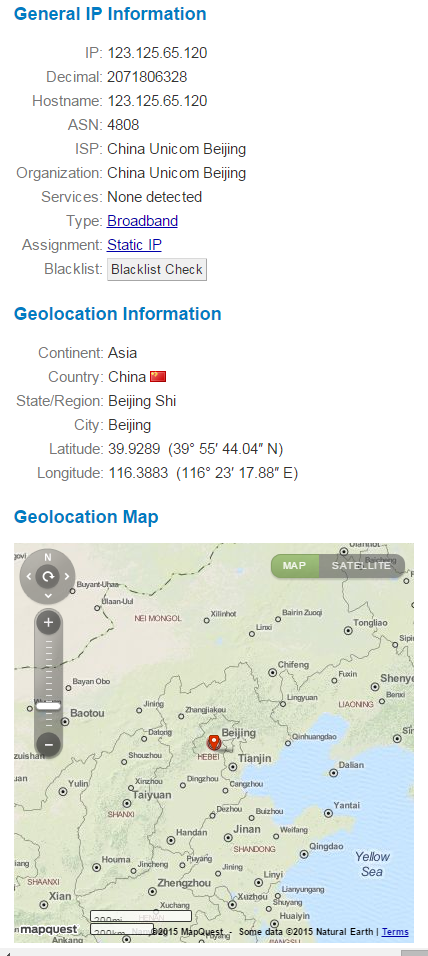
\includegraphics[width=\columnwidth]{figures/gfwbaiduip}
	\caption{
		Details on the destination IP address used in the experiments in \autoref{gfwbaseline} and \autoref{gfwlocation}.
		Note the location (Beijing) and the ISP (China Unicom).
	}
	\label{fig_gfwbaiduip}
\end{figure}

All of the requests prompted \texttt{Time-to-live exceeded} messages from intermediary nodes on the way to \texttt{123.125.65.120} until the request sent with TTL=24, which finally gets a \texttt{403} HTTP response (Figure \ref{fig_gfwtest}), as expected when requesting a google.com page from any server other than Google’s.
\begin{figure*}
	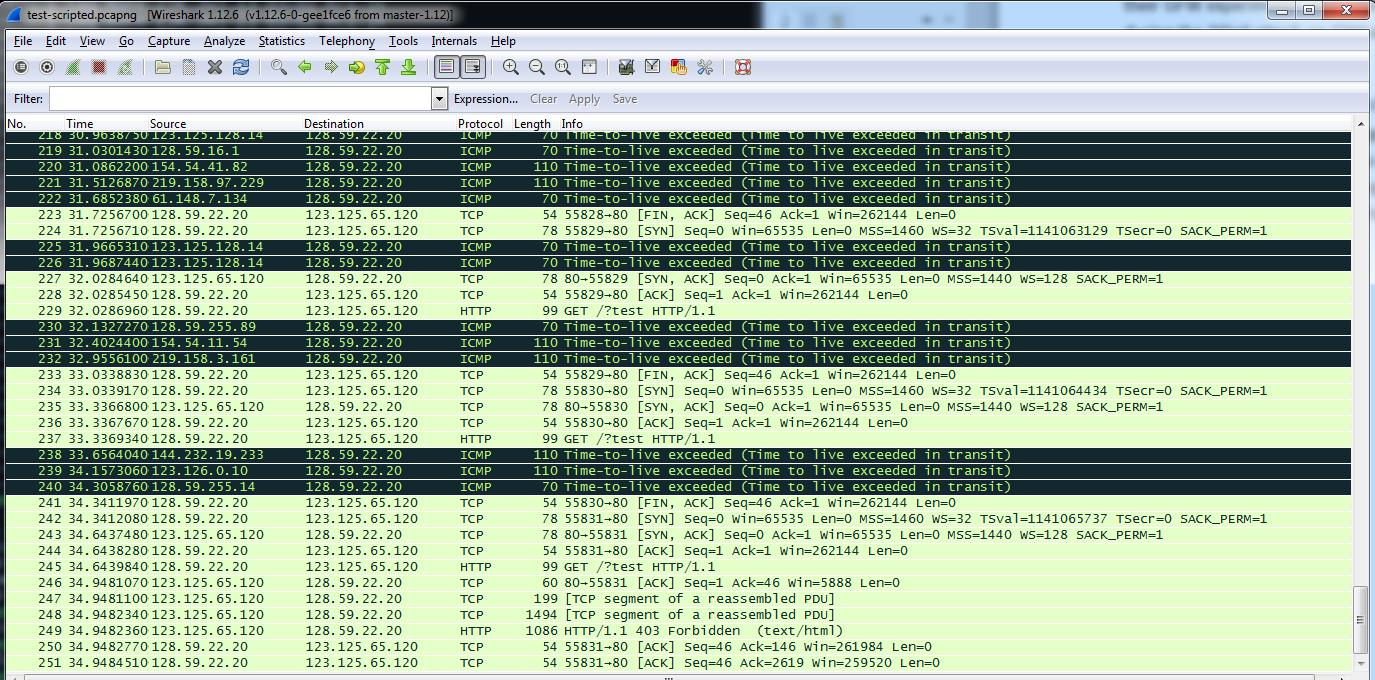
\includegraphics[width=\textwidth]{figures/gfwtest}
	\caption{
		No \texttt{[RST]} packets are sent when \texttt{www.google.com/?test} is requested from a Baidu server in Beijing.
		\texttt{Time-to-live exceeded} messages are received for small TTL values, until an HTTP response is received after sending the request with TTL=24 (packet 249), and the request reaches the Baidu server.
	}
	\label{fig_gfwtest}
\end{figure*}
The full packet capture can be found here: \url{https://github.com/tagatac/ttlprobe/blob/prelim/test-scripted.pcapng}.
The one spurious \texttt{[RST]} packet (packet 87) sent from my computer to \texttt{123.125.65.120} is a closing connection from a previous run of the same experiment.
You can see this from the port number used (55785), which is out of sequence with those from this experiment (55805--55831).
\subsubsection{GFW Location}\label{gfwlocation}
This experiment shows that the GFW is between 17 and 18 hops from my desktop along the path to \texttt{123.125.65.120}.
An identical experiment to Experiment 1 was performed, only substituting \texttt{falun} for \texttt{test} in the HTTP \texttt{GET} requests.
The results are the same as in \autoref{gfwbaseline} for TTL values 1--17.  For each TTL\textgreater=18, I received an \texttt{[RST]} packet and three \texttt{[RST, ACK]} packets apparently from \texttt{123.125.65.120} (but actually from GFW).
\texttt{[RST]} packets sent by the GFW to both endpoints (my desktop and the server and \texttt{123.125.65.120}) cause both to close the TCP connection.
The packet capture can be found here: \url{https://github.com/tagatac/ttlprobe/blob/prelim/falun-scripted.pcapng}.
The script used for both the experiments in \autoref{gfwbaseline} and \autoref{gfwlocation} can be found here: \url{https://github.com/tagatac/ttlprobe/blob/prelim/test.py}.
Figure \ref{fig_gfwfalun} shows the request with TTL=18 prompting the first \texttt{[RST]} packet from the GFW.
\begin{figure*}
	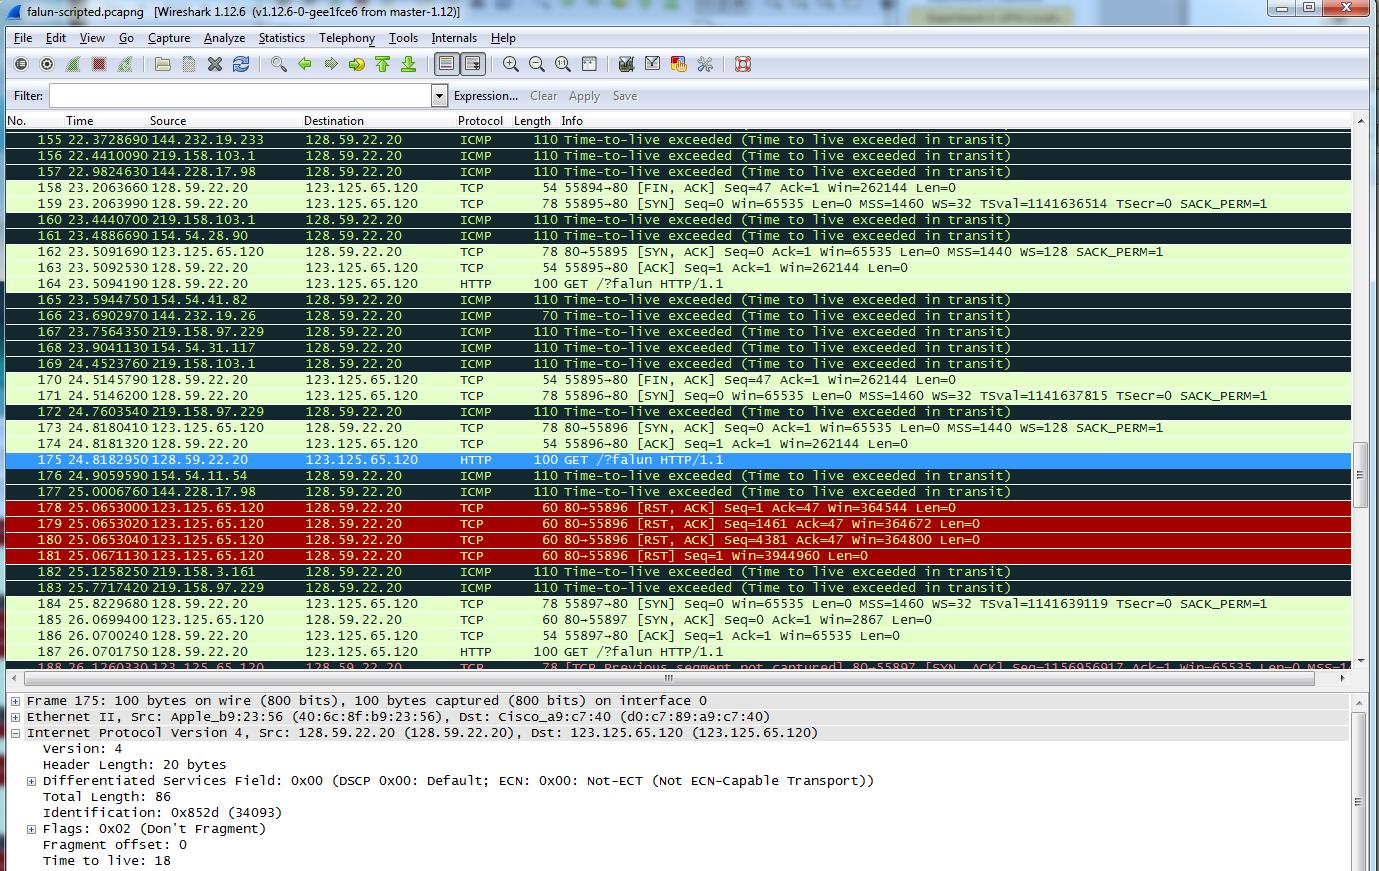
\includegraphics[width=\textwidth]{figures/gfwfalun}
	\caption{The GFW responds to the keywords \texttt{www.google.com/?falun} with several \texttt{[RST]} packets as soon as the request is sent 18 hops along the path to a Baidu server in Beijing.}
	\label{fig_gfwfalun}
\end{figure*}
\subsection{Probing for the Great Cannon}
\subsubsection{GitHub DDoS}
This experiment looked for GC packets as were observed during the DDoS on GitHub.
The observation specifically was a modified JavaScript file upon request for \texttt{hm.baidu.com/h.js}, an analytics tracking script similar to that used by Google Analytics.
The original can be found here: \url{https://github.com/tagatac/ttlprobe/blob/prelim/h.js}.
According to \mbox{NETRESEC}~\cite{Hjelmvik2015}, the modified file contains some obfuscated code that sends requests to GitHub in a 2-second loop.
Marczak et al. calculated that the substitution is made 1.75\% of the time, as long as your IP address is not ignored by the GC altogether, which happened to one of the machines they used for probing~\cite{Marczak2015}.
I ran a Python script (\url{https://github.com/tagatac/ttlprobe/blob/prelim/falunjs.py}) to download the analytics script for \texttt{7k7k.com} 1000 times.
MD5 hashes of every file match that of the unmodified JavaScript.